\documentclass[12pt,a4paper,oneside]{article}
\usepackage[dutch]{babel}
\usepackage{graphicx}
\usepackage{tikz}
\usepackage{a4wide}
\usepackage{amsmath}
\usepackage{amssymb}
\usepackage{rotating}
\usepackage{listings}
\usepackage{float}
\usepackage{color}
\usepackage{fancyhdr}
\definecolor{dkgreen}{rgb}{0,0.6,0}
\definecolor{gray}{rgb}{0.5,0.5,0.5}
\definecolor{mauve}{rgb}{0.58,0,0.82}
 
\lstset{ %
  language=PYTHON,                
  basicstyle=\footnotesize,           
  numbers=left,                  
  numberstyle=\tiny\color{gray},  
  stepnumber=2,                        
  numbersep=5pt,                  
  backgroundcolor=\color{white},      
  showspaces=false,               
  showstringspaces=false,        
  showtabs=false,                 
  frame=single,                   
  rulecolor=\color{black},        
  tabsize=2,                      
  captionpos=b,                   
  breaklines=true,                
  breakatwhitespace=false,        
  title=\lstname,                                                  
  keywordstyle=\color{blue},          
  commentstyle=\color{dkgreen},       
  stringstyle=\color{mauve},         
  escapeinside={\%*}{*)},            
  morekeywords={*,...},              
  deletekeywords={...}              
}

\begin{document}

\title{Codeereffici\"entie}
\author{Stefaan Vermassen}
\date{\today}
\pagestyle{fancy}
\fancyhf{}
\fancyhead[R]{Stefaan Vermassen}
\fancyhead[L]{Verslag DA3}
\fancyfoot[C]{\thepage}
\maketitle
\tableofcontents
\newpage
\begin{figure}[H]
  \begin{center}
    % GNUPLOT: LaTeX picture with Postscript
\begingroup
  \makeatletter
  \providecommand\color[2][]{%
    \GenericError{(gnuplot) \space\space\space\@spaces}{%
      Package color not loaded in conjunction with
      terminal option `colourtext'%
    }{See the gnuplot documentation for explanation.%
    }{Either use 'blacktext' in gnuplot or load the package
      color.sty in LaTeX.}%
    \renewcommand\color[2][]{}%
  }%
  \providecommand\includegraphics[2][]{%
    \GenericError{(gnuplot) \space\space\space\@spaces}{%
      Package graphicx or graphics not loaded%
    }{See the gnuplot documentation for explanation.%
    }{The gnuplot epslatex terminal needs graphicx.sty or graphics.sty.}%
    \renewcommand\includegraphics[2][]{}%
  }%
  \providecommand\rotatebox[2]{#2}%
  \@ifundefined{ifGPcolor}{%
    \newif\ifGPcolor
    \GPcolorfalse
  }{}%
  \@ifundefined{ifGPblacktext}{%
    \newif\ifGPblacktext
    \GPblacktexttrue
  }{}%
  % define a \g@addto@macro without @ in the name:
  \let\gplgaddtomacro\g@addto@macro
  % define empty templates for all commands taking text:
  \gdef\gplbacktext{}%
  \gdef\gplfronttext{}%
  \makeatother
  \ifGPblacktext
    % no textcolor at all
    \def\colorrgb#1{}%
    \def\colorgray#1{}%
  \else
    % gray or color?
    \ifGPcolor
      \def\colorrgb#1{\color[rgb]{#1}}%
      \def\colorgray#1{\color[gray]{#1}}%
      \expandafter\def\csname LTw\endcsname{\color{white}}%
      \expandafter\def\csname LTb\endcsname{\color{black}}%
      \expandafter\def\csname LTa\endcsname{\color{black}}%
      \expandafter\def\csname LT0\endcsname{\color[rgb]{1,0,0}}%
      \expandafter\def\csname LT1\endcsname{\color[rgb]{0,1,0}}%
      \expandafter\def\csname LT2\endcsname{\color[rgb]{0,0,1}}%
      \expandafter\def\csname LT3\endcsname{\color[rgb]{1,0,1}}%
      \expandafter\def\csname LT4\endcsname{\color[rgb]{0,1,1}}%
      \expandafter\def\csname LT5\endcsname{\color[rgb]{1,1,0}}%
      \expandafter\def\csname LT6\endcsname{\color[rgb]{0,0,0}}%
      \expandafter\def\csname LT7\endcsname{\color[rgb]{1,0.3,0}}%
      \expandafter\def\csname LT8\endcsname{\color[rgb]{0.5,0.5,0.5}}%
    \else
      % gray
      \def\colorrgb#1{\color{black}}%
      \def\colorgray#1{\color[gray]{#1}}%
      \expandafter\def\csname LTw\endcsname{\color{white}}%
      \expandafter\def\csname LTb\endcsname{\color{black}}%
      \expandafter\def\csname LTa\endcsname{\color{black}}%
      \expandafter\def\csname LT0\endcsname{\color{black}}%
      \expandafter\def\csname LT1\endcsname{\color{black}}%
      \expandafter\def\csname LT2\endcsname{\color{black}}%
      \expandafter\def\csname LT3\endcsname{\color{black}}%
      \expandafter\def\csname LT4\endcsname{\color{black}}%
      \expandafter\def\csname LT5\endcsname{\color{black}}%
      \expandafter\def\csname LT6\endcsname{\color{black}}%
      \expandafter\def\csname LT7\endcsname{\color{black}}%
      \expandafter\def\csname LT8\endcsname{\color{black}}%
    \fi
  \fi
  \setlength{\unitlength}{0.0500bp}%
  \begin{picture}(7200.00,5040.00)%
    \gplgaddtomacro\gplbacktext{%
      \csname LTb\endcsname%
      \put(946,704){\makebox(0,0)[r]{\strut{} 0.8}}%
      \csname LTb\endcsname%
      \put(946,1383){\makebox(0,0)[r]{\strut{} 1}}%
      \csname LTb\endcsname%
      \put(946,2061){\makebox(0,0)[r]{\strut{} 1.2}}%
      \csname LTb\endcsname%
      \put(946,2739){\makebox(0,0)[r]{\strut{} 1.4}}%
      \csname LTb\endcsname%
      \put(946,3418){\makebox(0,0)[r]{\strut{} 1.6}}%
      \csname LTb\endcsname%
      \put(946,4096){\makebox(0,0)[r]{\strut{} 1.8}}%
      \csname LTb\endcsname%
      \put(946,4775){\makebox(0,0)[r]{\strut{} 2}}%
      \csname LTb\endcsname%
      \put(1651,484){\makebox(0,0){\strut{} 5}}%
      \csname LTb\endcsname%
      \put(3082,484){\makebox(0,0){\strut{} 10}}%
      \csname LTb\endcsname%
      \put(4513,484){\makebox(0,0){\strut{} 15}}%
      \csname LTb\endcsname%
      \put(5944,484){\makebox(0,0){\strut{} 20}}%
      \put(176,2739){\rotatebox{-270}{\makebox(0,0){\strut{}Relatieve oplossing}}}%
      \put(3940,154){\makebox(0,0){\strut{}Aantal steden}}%
    }%
    \gplgaddtomacro\gplfronttext{%
      \csname LTb\endcsname%
      \put(5302,4602){\makebox(0,0)[r]{\strut{}optimale kost}}%
      \csname LTb\endcsname%
      \put(5302,4382){\makebox(0,0)[r]{\strut{}simulated annealing}}%
      \csname LTb\endcsname%
      \put(5302,4162){\makebox(0,0)[r]{\strut{}simulated annealing+tabu search}}%
    }%
    \gplbacktext
    \put(0,0){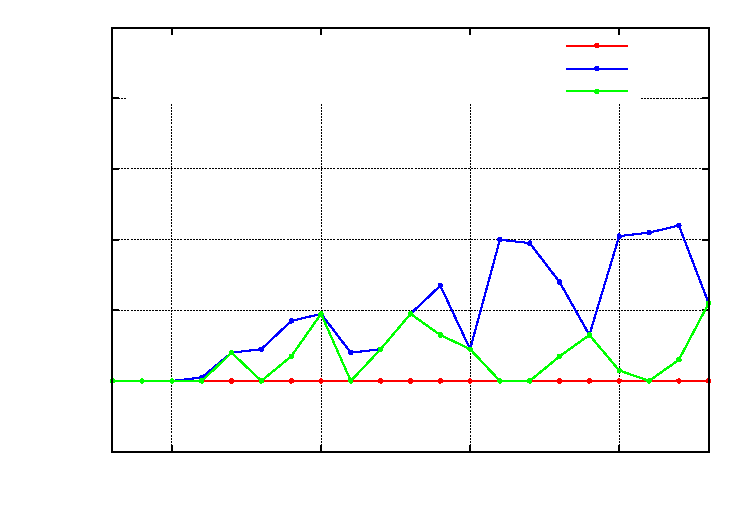
\includegraphics{testresults/afwijking-eps-converted-to.pdf}}%
    \gplfronttext
  \end{picture}%
\endgroup

    \caption{1.000.000 toevoegbewerkingen en 10.000.000 opzoekbewerkingen}
    \label{graph:graph1}
  \end{center}
\end{figure}
\end{document}